\documentclass{article}
\usepackage[margin=1in]{geometry}
\usepackage{array}
\usepackage{amsmath}
\usepackage{amssymb}
\usepackage{booktabs}
\usepackage{longtable}
\usepackage{float}
\usepackage{tikz}
\usepackage{pgfplots}
\usepackage{caption}
\usepackage{xcolor}
\usetikzlibrary{arrows.meta,positioning,calc,fit,backgrounds}
\pgfplotsset{compat=1.18}

\InputIfFileExists{report-header.tex}{}{
    \newcommand{\TeamName}{Team name here}
    \newcommand{\MemberOne}{Member 1 name here}
    \newcommand{\MemberOneCode}{Member 1 code here}
    \newcommand{\MemberTwo}{Member 2 name here}
    \newcommand{\MemberTwoCode}{Member 2 code here}
    \newcommand{\MemberThree}{Member 3 name here}
    \newcommand{\MemberThreeCode}{Member 3 code here}
    \newcommand{\MemberFour}{Member 4 name here}
    \newcommand{\MemberFourCode}{Member 4 code here}
}

\begin{document}

\begin{center}
\section*{Problem Session 9: Replacement Algorithm}
\textbf{CPE223 Computer Architecture}\\
\textbf{Team: \TeamName}\\
\textit{\MemberOne\ (\MemberOneCode)}\\
\textit{\MemberTwo\ (\MemberTwoCode)}\\
\textit{\MemberThree\ (\MemberThreeCode)}\\
\textit{\MemberFour\ (\MemberFourCode)}
\end{center}

\section*{1. Problem Statement}
The cache contains 8 blocks and each block stores one 16-bit word. The memory address width is 16 bits. The array $A(4,10)$ is stored in column-major order. The program first computes the sum and average of the first row, then normalizes each element of that row:

\begin{align*}
\texttt{SUM} &\leftarrow 0 \\
\texttt{for } j &= 0 \texttt{ to } 9: \quad \texttt{SUM} \leftarrow \texttt{SUM} + A(0,j) \\
\texttt{AVE} &\leftarrow \texttt{SUM}/10 \\
\texttt{for } i &= 9 \texttt{ downto } 0: \quad A(0,i) \leftarrow A(0,i) / \texttt{AVE}
\end{align*}

This report tracks how the cache evolves under LRU replacement for two mapping schemes:
\begin{itemize}
    \item Fully associative mapping with tag = 16 bits, word = 0 bits.
    \item Set associative mapping exactly as written in the assignment: tag = 15 bits, set = 1 bit, word = 0 bits.
\end{itemize}

\section*{2. Assumptions and Address Derivation}
We assume the base word address of $A(0,0)$ is 0. Since each cache block stores exactly one word and the problem states word = 0, there is no block offset field.

For a column-major array $A(4,10)$, the word address offset is
\[
\text{offset}(A(i,j)) = i + 4j.
\]
For the first row, $i=0$, so
\[
\text{offset}(A(0,j)) = 4j.
\]
Therefore, the addresses used by the program are
\[
0,\ 4,\ 8,\ 12,\ 16,\ 20,\ 24,\ 28,\ 32,\ 36.
\]
The full reference string is
\[
0,4,8,12,16,20,24,28,32,36,36,32,28,24,20,16,12,8,4,0.
\]

\begin{figure}[H]
\centering
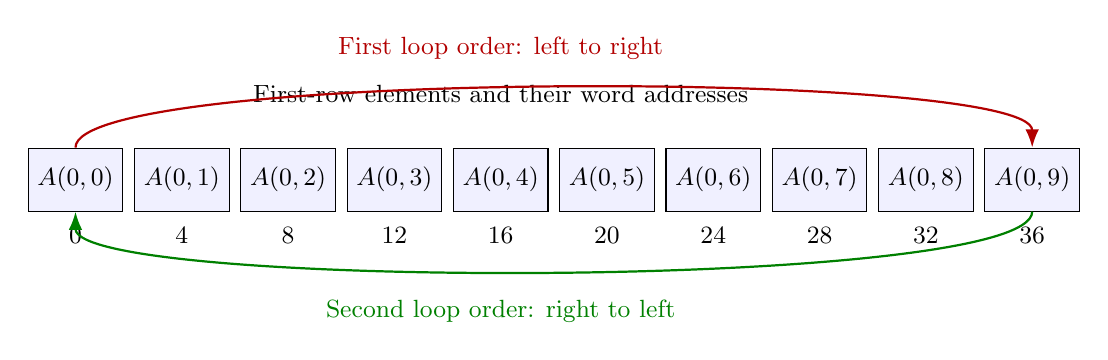
\begin{tikzpicture}[>=Latex, every node/.style={font=\small}]
\foreach \j/\addr in {0/0,1/4,2/8,3/12,4/16,5/20,6/24,7/28,8/32,9/36} {
    \node[draw, minimum width=1.1cm, minimum height=0.8cm, fill=blue!6] (c\j) at (1.35*\j,0) {$A(0,\j)$};
    \node[below=2pt of c\j] {\addr};
}
\node[above=0.45cm of c4] {First-row elements and their word addresses};
\draw[thick,->,red!70!black] (c0.north) .. controls +(0,1.0) and +(0,1.0) .. (c9.north);
\node[red!70!black, above=1.0cm of c4] {First loop order: left to right};
\draw[thick,->,green!50!black] (c9.south) .. controls +(0,-1.0) and +(0,-1.0) .. (c0.south);
\node[green!50!black, below=1.0cm of c4] {Second loop order: right to left};
\end{tikzpicture}
\caption{Memory layout of the accessed first-row elements in column-major storage.}
\end{figure}

\section*{3. Cache Mapping Rules}

\subsection*{3.1 Fully Associative Mapping}
All 8 cache lines belong to one replacement group. Any memory block can be stored in any line. The LRU policy is global across the whole cache.

\subsection*{3.2 Set Associative Mapping from the Assignment}
The assignment specifies tag = 15 bits and set = 1 bit. This implies 2 sets total. Since the cache has 8 blocks, each set contains 4 lines. The set index is the least significant address bit:
\[
\text{set} = \text{address} \bmod 2.
\]
Because every referenced address is even, every access goes to Set 0 and Set 1 is never used.

\begin{figure}[H]
\centering
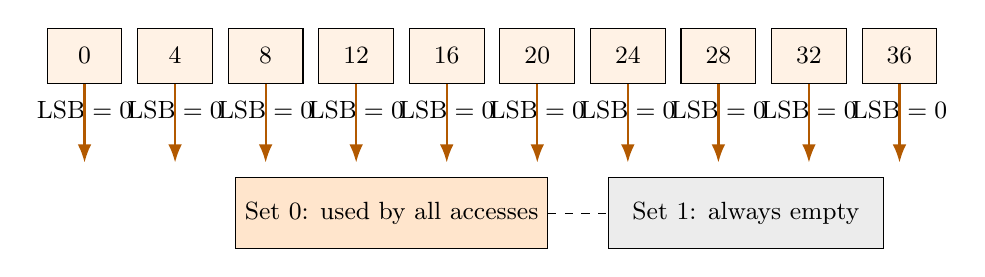
\begin{tikzpicture}[node distance=0.55cm and 0.9cm, >=Latex, every node/.style={font=\small}]
\foreach \k/\a in {0/0,1/4,2/8,3/12,4/16,5/20,6/24,7/28,8/32,9/36} {
    \node[draw, minimum width=0.95cm, minimum height=0.7cm, fill=orange!10] (a\k) at (1.15*\k,0) {\a};
    \node[below=0.1cm of a\k] {$\text{LSB}=0$};
    \draw[->,thick,orange!70!black] (a\k.south) -- ++(0,-1.0);
}
\node[draw, minimum width=3.5cm, minimum height=0.9cm, fill=orange!20] (s0) at (3.9,-2.0) {Set 0: used by all accesses};
\node[draw, minimum width=3.5cm, minimum height=0.9cm, fill=gray!15] (s1) at (8.4,-2.0) {Set 1: always empty};
\draw[dashed] (s0.east) -- (s1.west);
\end{tikzpicture}
\caption{All referenced addresses are even, so every access maps to Set 0.}
\end{figure}

\section*{4. Fully Associative LRU Simulation}
Cache content is written from most recently used (MRU) to least recently used (LRU). To keep the table aligned, each cache position is shown in its own subcolumn.

\scriptsize
\setlength{\tabcolsep}{3.5pt}
\begin{longtable}{@{}cclcc*{8}{c}@{}}
\toprule
& & & & & \multicolumn{8}{c}{Cache After Access (MRU $\rightarrow$ LRU)} \\
\cmidrule(l){6-13}
Step & Loop & Access & Address & Hit/Miss & 1 & 2 & 3 & 4 & 5 & 6 & 7 & 8 \\
\midrule
\endhead
1 & $j=0$ & $A(0,0)$ & 0 & Miss & 0 & - & - & - & - & - & - & - \\
2 & $j=1$ & $A(0,1)$ & 4 & Miss & 4 & 0 & - & - & - & - & - & - \\
3 & $j=2$ & $A(0,2)$ & 8 & Miss & 8 & 4 & 0 & - & - & - & - & - \\
4 & $j=3$ & $A(0,3)$ & 12 & Miss & 12 & 8 & 4 & 0 & - & - & - & - \\
5 & $j=4$ & $A(0,4)$ & 16 & Miss & 16 & 12 & 8 & 4 & 0 & - & - & - \\
6 & $j=5$ & $A(0,5)$ & 20 & Miss & 20 & 16 & 12 & 8 & 4 & 0 & - & - \\
7 & $j=6$ & $A(0,6)$ & 24 & Miss & 24 & 20 & 16 & 12 & 8 & 4 & 0 & - \\
8 & $j=7$ & $A(0,7)$ & 28 & Miss & 28 & 24 & 20 & 16 & 12 & 8 & 4 & 0 \\
9 & $j=8$ & $A(0,8)$ & 32 & Miss & 32 & 28 & 24 & 20 & 16 & 12 & 8 & 4 \\
10 & $j=9$ & $A(0,9)$ & 36 & Miss & 36 & 32 & 28 & 24 & 20 & 16 & 12 & 8 \\
11 & $i=9$ & $A(0,9)$ & 36 & Hit & 36 & 32 & 28 & 24 & 20 & 16 & 12 & 8 \\
12 & $i=8$ & $A(0,8)$ & 32 & Hit & 32 & 36 & 28 & 24 & 20 & 16 & 12 & 8 \\
13 & $i=7$ & $A(0,7)$ & 28 & Hit & 28 & 32 & 36 & 24 & 20 & 16 & 12 & 8 \\
14 & $i=6$ & $A(0,6)$ & 24 & Hit & 24 & 28 & 32 & 36 & 20 & 16 & 12 & 8 \\
15 & $i=5$ & $A(0,5)$ & 20 & Hit & 20 & 24 & 28 & 32 & 36 & 16 & 12 & 8 \\
16 & $i=4$ & $A(0,4)$ & 16 & Hit & 16 & 20 & 24 & 28 & 32 & 36 & 12 & 8 \\
17 & $i=3$ & $A(0,3)$ & 12 & Hit & 12 & 16 & 20 & 24 & 28 & 32 & 36 & 8 \\
18 & $i=2$ & $A(0,2)$ & 8 & Hit & 8 & 12 & 16 & 20 & 24 & 28 & 32 & 36 \\
19 & $i=1$ & $A(0,1)$ & 4 & Miss & 4 & 8 & 12 & 16 & 20 & 24 & 28 & 32 \\
20 & $i=0$ & $A(0,0)$ & 0 & Miss & 0 & 4 & 8 & 12 & 16 & 20 & 24 & 28 \\
\bottomrule
\caption{Fully associative cache evolution under LRU.}
\end{longtable}
\normalsize

Summary:
\begin{itemize}
    \item Hits = 8
    \item Misses = 12
    \item Hit rate = 40\%
\end{itemize}

The first 8 accesses fill the cache. Accesses to 32 and 36 replace the two oldest blocks, which are 0 and 4. During the reverse loop, addresses from 36 down to 8 are still resident, so they hit. The final two accesses miss because those blocks were already replaced.

\section*{5. Set Associative LRU Simulation}
The cache has 2 sets with 4 lines per set. LRU is maintained separately inside each set. The cache state is split into subcolumns so each line position stays aligned.

\scriptsize
\setlength{\tabcolsep}{3.5pt}
\begin{longtable}{@{}cclcc*{8}{c}@{}}
\toprule
& & & & & \multicolumn{4}{c}{Set 0 After Access (MRU $\rightarrow$ LRU)} & \multicolumn{4}{c}{Set 1 After Access (MRU $\rightarrow$ LRU)} \\
\cmidrule(l){6-9}\cmidrule(l){10-13}
Step & Loop & Access & Address & Hit/Miss & 1 & 2 & 3 & 4 & 1 & 2 & 3 & 4 \\
\midrule
\endhead
1 & $j=0$ & $A(0,0)$ & 0 & Miss & 0 & - & - & - & - & - & - & - \\
2 & $j=1$ & $A(0,1)$ & 4 & Miss & 4 & 0 & - & - & - & - & - & - \\
3 & $j=2$ & $A(0,2)$ & 8 & Miss & 8 & 4 & 0 & - & - & - & - & - \\
4 & $j=3$ & $A(0,3)$ & 12 & Miss & 12 & 8 & 4 & 0 & - & - & - & - \\
5 & $j=4$ & $A(0,4)$ & 16 & Miss & 16 & 12 & 8 & 4 & - & - & - & - \\
6 & $j=5$ & $A(0,5)$ & 20 & Miss & 20 & 16 & 12 & 8 & - & - & - & - \\
7 & $j=6$ & $A(0,6)$ & 24 & Miss & 24 & 20 & 16 & 12 & - & - & - & - \\
8 & $j=7$ & $A(0,7)$ & 28 & Miss & 28 & 24 & 20 & 16 & - & - & - & - \\
9 & $j=8$ & $A(0,8)$ & 32 & Miss & 32 & 28 & 24 & 20 & - & - & - & - \\
10 & $j=9$ & $A(0,9)$ & 36 & Miss & 36 & 32 & 28 & 24 & - & - & - & - \\
11 & $i=9$ & $A(0,9)$ & 36 & Hit & 36 & 32 & 28 & 24 & - & - & - & - \\
12 & $i=8$ & $A(0,8)$ & 32 & Hit & 32 & 36 & 28 & 24 & - & - & - & - \\
13 & $i=7$ & $A(0,7)$ & 28 & Hit & 28 & 32 & 36 & 24 & - & - & - & - \\
14 & $i=6$ & $A(0,6)$ & 24 & Hit & 24 & 28 & 32 & 36 & - & - & - & - \\
15 & $i=5$ & $A(0,5)$ & 20 & Miss & 20 & 24 & 28 & 32 & - & - & - & - \\
16 & $i=4$ & $A(0,4)$ & 16 & Miss & 16 & 20 & 24 & 28 & - & - & - & - \\
17 & $i=3$ & $A(0,3)$ & 12 & Miss & 12 & 16 & 20 & 24 & - & - & - & - \\
18 & $i=2$ & $A(0,2)$ & 8 & Miss & 8 & 12 & 16 & 20 & - & - & - & - \\
19 & $i=1$ & $A(0,1)$ & 4 & Miss & 4 & 8 & 12 & 16 & - & - & - & - \\
20 & $i=0$ & $A(0,0)$ & 0 & Miss & 0 & 4 & 8 & 12 & - & - & - & - \\
\bottomrule
\caption{Set associative cache evolution under LRU with the assignment's 1-bit set field.}
\end{longtable}
\normalsize

Summary:
\begin{itemize}
    \item Hits = 4
    \item Misses = 16
    \item Hit rate = 20\%
\end{itemize}

This cache behaves like a 4-line effective cache for this program because all references collide in Set 0. Set 1 remains empty during the entire execution.

\section*{6. Visual Comparison}

\begin{figure}[H]
\centering
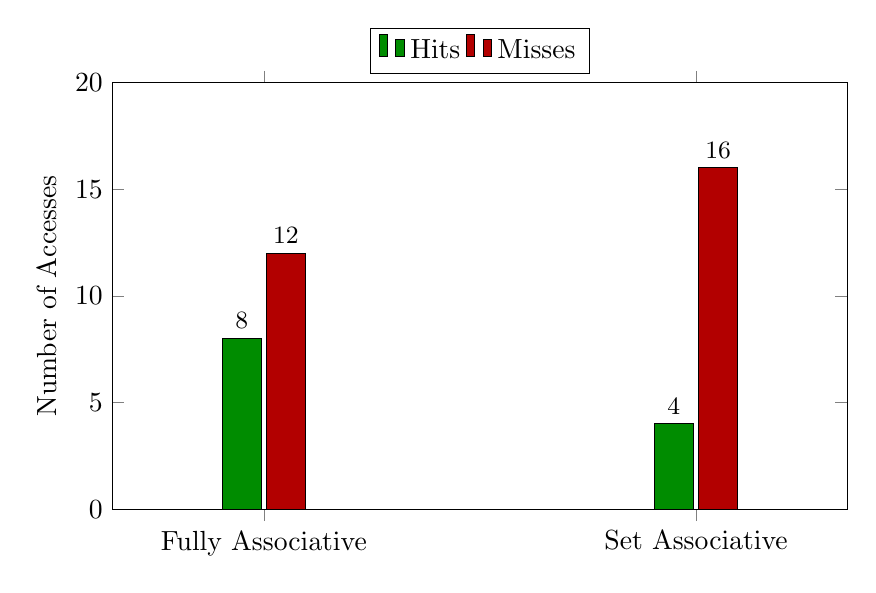
\begin{tikzpicture}
\begin{axis}[
    ybar,
    bar width=14pt,
    width=0.9\textwidth,
    height=7cm,
    ylabel={Number of Accesses},
    symbolic x coords={Fully Associative,Set Associative},
    xtick=data,
    ymin=0,
    ymax=20,
    enlarge x limits=0.35,
    legend style={at={(0.5,1.02)},anchor=south,legend columns=2},
    nodes near coords,
    every node near coord/.append style={font=\small}
]
\addplot[fill=green!55!black] coordinates {(Fully Associative,8) (Set Associative,4)};
\addplot[fill=red!70!black] coordinates {(Fully Associative,12) (Set Associative,16)};
\legend{Hits,Misses}
\end{axis}
\end{tikzpicture}
\caption{Hit and miss comparison between the two mapping schemes.}
\end{figure}

\begin{figure}[H]
\centering
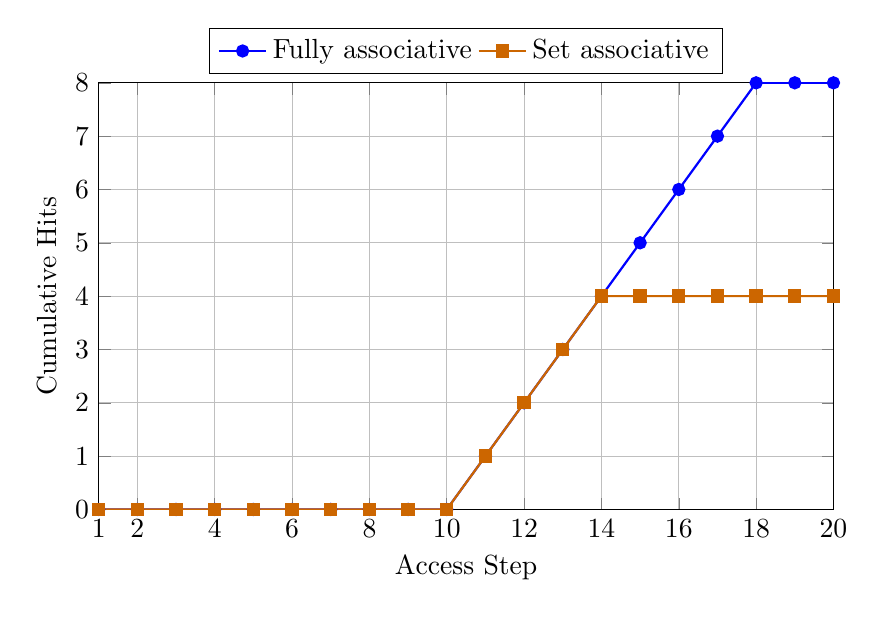
\begin{tikzpicture}
\begin{axis}[
    width=0.9\textwidth,
    height=7cm,
    xlabel={Access Step},
    ylabel={Cumulative Hits},
    xmin=1, xmax=20,
    ymin=0, ymax=8,
    xtick={1,2,4,6,8,10,12,14,16,18,20},
    ytick={0,1,2,3,4,5,6,7,8},
    legend style={at={(0.5,1.02)},anchor=south,legend columns=2},
    grid=both
]
\addplot[thick,blue,mark=*] coordinates {
    (1,0) (2,0) (3,0) (4,0) (5,0) (6,0) (7,0) (8,0) (9,0) (10,0)
    (11,1) (12,2) (13,3) (14,4) (15,5) (16,6) (17,7) (18,8) (19,8) (20,8)
};
\addplot[thick,orange!80!black,mark=square*] coordinates {
    (1,0) (2,0) (3,0) (4,0) (5,0) (6,0) (7,0) (8,0) (9,0) (10,0)
    (11,1) (12,2) (13,3) (14,4) (15,4) (16,4) (17,4) (18,4) (19,4) (20,4)
};
\legend{Fully associative, Set associative}
\end{axis}
\end{tikzpicture}
\caption{Cumulative hit count over time. The fully associative cache continues to benefit deeper into the reverse loop.}
\end{figure}

\section*{7. Discussion}
The fully associative cache performs better because all 8 lines can be used by the 10-word working set. After the first loop, only two addresses have been evicted, so most accesses in the reverse loop hit.

The set associative design performs worse under the literal assignment parameters because the 1-bit set index depends on address parity. Since all references are even, they all map to Set 0. This creates continuous conflict within one 4-line set while the other 4 lines in Set 1 remain unused. The result is a lower hit rate even though the total cache still has 8 lines.

\section*{8. Conclusion}
For this access pattern, fully associative LRU gives 8 hits and 12 misses, for a 40\% hit rate. The set associative cache defined by the assignment gives 4 hits and 16 misses, for a 20\% hit rate. The difference is caused entirely by the address distribution: all accessed words have least significant bit 0, so the set associative design effectively behaves as a 4-line cache.

\section*{Appendix: PowerPoint Animation Notes}
To create the required animation in PowerPoint, use the simulation tables directly. Duplicate one table frame for each step, update the access and cache content, and apply a simple fade or appear animation between frames. The two figures in this report are also useful as overview slides before the per-step animation.

\end{document}
